% !TEX TS-program = pdflatex
% !TEX encoding = UTF-8 Unicode

% This is a simple template for a LaTeX document using the "article" class.
% See "book", "report", "letter" for other types of document.

\documentclass[11pt]{article} % use larger type; default would be 10pt

\usepackage[utf8]{inputenc} % set input encoding (not needed with XeLaTeX)

%%% Examples of Article customizations

%%% PAGE DIMENSIONS
\usepackage{geometry} % to change the page dimensions
\geometry{a4paper} % or letterpaper (US) or a5paper or....
% \geometry{margin=2in} % for example, change the margins to 2 inches all round
% \geometry{landscape} % set up the page for landscape
%   read geometry.pdf for detailed page layout information

\usepackage{graphicx} % support the \includegraphics command and options

% \usepackage[parfill]{parskip} % Activate to begin paragraphs with an empty line rather than an indent

%%% PACKAGES
\usepackage{booktabs} % for much better looking tables
\usepackage{array} % for better arrays (eg matrices) in maths
\usepackage{paralist} % very flexible & customisable lists (eg. enumerate/itemize, etc.)
\usepackage{verbatim} % adds environment for commenting out blocks of text & for better verbatim
\usepackage{multicol,caption}
\usepackage{wrapfig}
\usepackage{parskip}
\usepackage{arydshln}
\usepackage{amsfonts}
\usepackage{amsmath}
% These packages are all incorporated in the memoir class to one degree or another...

%%% HEADERS & FOOTERS
\usepackage{fancyhdr} % This should be set AFTER setting up the page geometry
\pagestyle{fancy} % options: empty , plain , fancy
\renewcommand{\headrulewidth}{0pt} % customise the layout...
\lhead{}\chead{}\rhead{}
\lfoot{}\cfoot{\thepage}\rfoot{}

%%% SECTION TITLE APPEARANCE
\usepackage{sectsty}
\allsectionsfont{\sffamily\mdseries\upshape} % (See the fntguide.pdf for font help)
% (This matches ConTeXt defaults)

%%% ToC (table of contents) APPEARANCE
\usepackage[nottoc,notlof,notlot]{tocbibind} % Put the bibliography in the ToC
\usepackage[titles,subfigure]{tocloft} % Alter the style of the Table of Contents

\renewcommand{\cftsecfont}{\rmfamily\mdseries\upshape}
\renewcommand{\cftsecpagefont}{\rmfamily\mdseries\upshape} % No bold!
\newcommand{\squeezeup}{\vspace{-25pt}}

%%% Object appearance
\usepackage{float, makecell}
\usepackage{subcaption}
\newenvironment{Figure}{\par\medskip\noindent\minipage{\linewidth}}{\endminipage\par\medskip}
\newenvironment{Table}{\par\smallskip\noindent\minipage{\linewidth}}{\endminipage\par\smallskip}
\usepackage[linewidth=0.01pt,linecolor=black]{mdframed}
\captionsetup{justification=raggedright,singlelinecheck=false}

%%% END Article customizations

%%% Document content

\title{Homework 1 : Unsupervised Deep Learning}
\author{João Ramos da Silva Tabuaço Freitas \\ Università Degli Studi di Padova \\ Student ID: 2009440}
\date{18 July 2022} %Display a given date

\begin{document}
\maketitle

\section*{Introduction}
Unsupervised learning takes an agnostic approach in learning features in data. This distinguishes it from supervised learning, where models attempt to form a connection between an input and a ground-truth target. The performance of unsupervised learning models is normally assessed by how faithfully the data can be reproduced from the features learned.

\textbf{Autoencoders} and \textbf{generative-adversarial networks} (GANs) are two models used in unsupervised learning. In both cases, these models are composed by a perception module along with a reproduction module. These two work in tandem to achieve faithful reproduction of data with large number of features.

\noindent The goal of the autoencoder $A$ is to learn to embed input data $\mathbf{x}$ in a latent space $\mathbb{R}^{n}$ of reduced dimensionality, and subsequently reproduce it. To achieve this, an encoder $E$ transforms an input into a single vector in said latent space $z = E(x), z \in \mathbb{R}^{n}$. A decoder $D$ then attempts to reproduce the original input $\mathbf{x}' = D(z)$ as faithfully as possible. This motivates the use of mean-squared error (MSE) to quantify the reconstruction error.

\begin{equation}
    \{\hat{w}\}= \arg\min_{w} \frac{1}{n}\sum_{i = 1}^{n}\left(\hat{\mathbf{x}}_i - \mathbf{x}_i\right)^{2}
\end{equation}

\noindent Of course, the autoencoder $A := D \circ E$.

\noindent Autoencoders with a latent space of lower dimension than the input space are said to be undercomplete, while those with a larger latent space are overcomplete. Evidently, the former performs dimensionality reduction, by learning only data's most prominent features. This proves useful in denoising input, for example. While the latter could have the capability of capturing larger detail from the inputs, its learning converges to the identity. In a denoising scenario, this means the output will be just as noisy as the input. This is simply a consequence of using reconstruction error as the learning criterion.

\noindent The performance of an undercomplete autoencoder can be compared with principal component analysis (PCA), or t-distributed stochastic neighbor embedding (t-SNE) on the input data. In fact, an autoencoder without non-linearities is expected to learn the structure of a PCA subspace. Naturally, non-linearity aids in capturing a more diverse set of features, which arguably endows the autoencoder with a larger descriptive power. To test this, its performance may be compared to t-SNE, which is well-established as a non-linear method of dimensionality reduction.

\noindent The structure of a GAN differs slightly from that of an autoencoder. It starts with a generator which produces samples $\mathbf{x} = g(\mathbf{z},w_{g})$ from a randomly generated latent vector $\mathbf{z}$, where $w_{g}$ are the generator parameters. These samples are then fed into the discriminator, whose goal is to observe an input, and reach a conclusion $y = d(\mathbf{x}, w_{d}) = d(g(\mathbf{z},w_{g}), w_{d})$ about said input (with $w_{d}$ being the discriminator parameters). The learning task can be formulated as a zero-sum game solved by a minimax decision.\footnote{Goodfellow, I. J., Pouget-Abadie, J., Mirza, M., Xu, B., Warde-Farley, D., Ozair, S.,
Courville, A., and Bengio, Y. (2014c). Generative adversarial networks. In NIPS’2014.} The discriminator observes a payoff $v(g, d)$, while the generator receives $-v(g,d)$. Thus, the goal is to find $g^*$ such that:

\begin{equation}
    g^* = \arg\min_{g}\max_{d} v(g,d)
\end{equation}

Normally, the choice of $v(g, d)$ is:
\begin{equation}
    v_{\text{mm}}(g,d) = - \mathbb{E}_{\mathbf{x}\sim p_{\text{data}}}[\log(d(\mathbf{x}))] - \mathbb{E}_{\mathbf{x}\sim p_{g}}[\log(1 - d(\mathbf{x}))]
\end{equation}

In other words, the aim of the minimax game is for the discriminator to maximize its payoff by classifying fake/real inputs correctly, while the generator attempts to minimize the discriminator's payoff by tricking it into believing that the inputs are real.

\noindent One issue with the minimax game formulation is that the gradient quickly diverges away from $d(\mathbf{x}) = 1/2$. This can be addressed by modifying the generator loss, as is done in non-saturating GAN (NSGAN) formulation.\footnote{Lucic, M., Kurach, K., Michalski, M., Bousquet, O., Gelly, S.,  (2018). Are GANs Created Equal? A Large-Scale Study. In NIPS'2018.} In this scenario, the discriminator loss is $v_{\text{mm}}$, while the generator loss is:
\begin{equation}
    v_{\text{NS}}(g,d) = - \mathbb{E}_{\mathbf{x}\sim p_{g}}[\log(d(\mathbf{x}))]
\end{equation}

Both the minimax and the non-saturating formulations will be explored.

%%%%%%%%%%%%%%  Methods section %%%%%%%%%%%%%%
\section*{Methods}

The FashionMNIST dataset is used to explore both the autoencoder and the GAN, with each image having shape $\left(1, 28, 28\right)$. The set used for training consisted of $60000$ equally distributed samples, which was sectioned to serve the purpose of validation as well. The test set consists of $10000$ samples with the same properties. 
 
The autoencoder architecture consists of three convolutional layers, followed by two fully connected layers. Regularization is implemented through batch normalization on the convolutional layers, and L2 penalty on the loss. The number of convolutional filters, number of fully-connected neurons, optimizer algorithm, and learning rate are tuned using Optuna, which attempted $20$ sets of parameters, training each model over five epochs. The latent space dimension is also tuned, but kept below $15$ to maintain the model undercomplete. However, dimensionality reduction is explored using latent dimension $\text{dim}(z) = 2$ for ease of visualization. The convolutional kernel sizes, strides and padding are kept constant to preserve the same output shapes in all trials. While different values for these could be attempted, preliminary attempts showed no discernible difference in training convergence or model performance.

\noindent Upon tuning the model architecture, the model was validated using a K-Fold cross-validation strategy, splitting the dataset in six sequential folds and performing training over $20$ epochs. The performance was assessed based on the reconstruction error on the test set.

\noindent To test the expressive power of the model, a convolutional neural network was trained to classify the set of latent vectors corresponding to the input data. The network's learning curve was compared to a similar network trained on the unaltered dataset, over $50$ epochs.

\noindent Finally, a new encoder's dimensionality reduction was visually compared to PCA and t-SNE. A perfect encoder would be able to spatially separate the data points in the latent space. Of course, some confusion is expected between some classes of similar-looking items, both for the encoder and the other methods.

\noindent The creation and training of the GAN posed several challenges. The level of complexity of the model discouraged hyperparameter tuning. This was because the Optuna framework would have to explore the hyperparameter space based on two different metrics (generator and discriminator loss). The set of parameters which would improve the generator performance could hinder the discriminator's, and vice-versa. Because of this, automated tuning was not performed. Furthermore, the training process revealed itself demanding from a computational standpoint. As a result, only one model was trained without cross-validation. Given the well-known regularity of the FashionMNIST dataset, this is acceptable, as there are no large disparities in different sections of the dataset.

\noindent Both components of the GAN were endowed with four convolutional layers, and no fully-connected section. The number of filters, kernel sizes, strides, and padding were chosen in order to have the generator outputting an image with the same dimensions as the FashionMNIST inputs, and the discriminator outputting a single scalar value.

\section*{Results}

\noindent The best architecture found for the autoencoder is described in Table 1. The K-fold results (Figure 1) show little variability in the learning curves, which is expected by the fairly regular nature and even distribution of class labels in the dataset. While the training loss experiences larger variance, the trend is similar for training and validation across all folds. The convergence of training and validation loss close to 20 training epochs indicates the model is well-regularized and not overfitting.

\noindent The denoising capabilities of the autoencoder were tested by inputting an image with different levels of noise. The results (Figure 2) show that the model is capable of reconstructing images rather well.

\begin{wrapfigure}{r}{4cm}
    \centering
    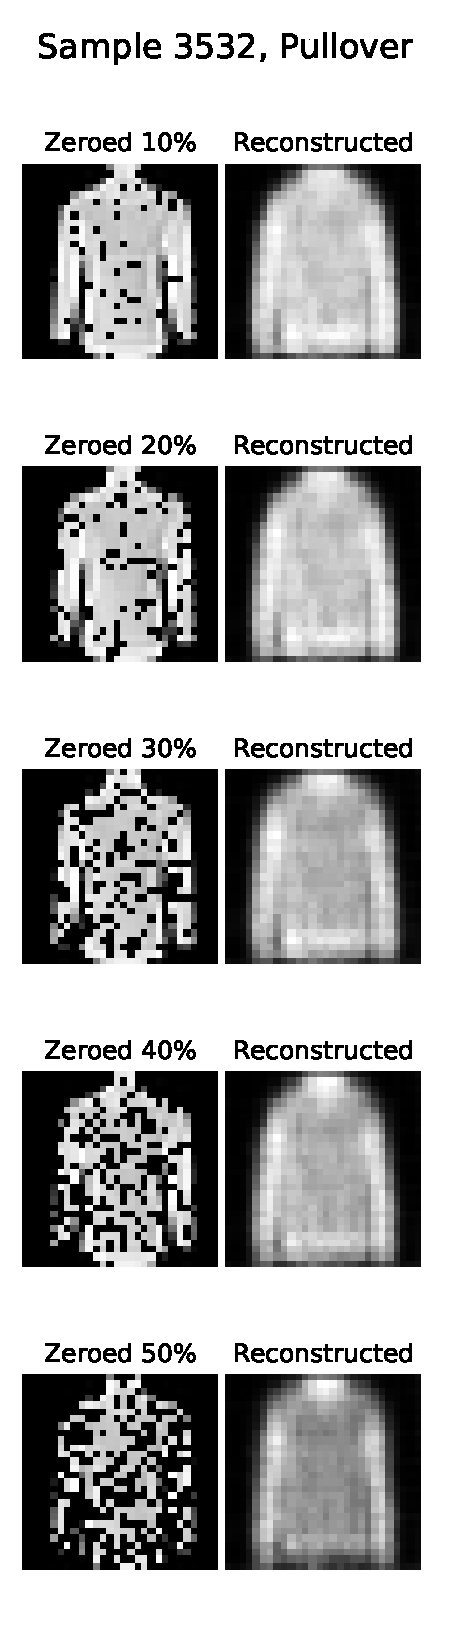
\includegraphics[height=0.5\textwidth]{res/Reconstruction.pdf}
    \caption{Noisy sample reconstruction}
    \end{wrapfigure}

\begin{wrapfigure}{r}{11cm}
    \centering
    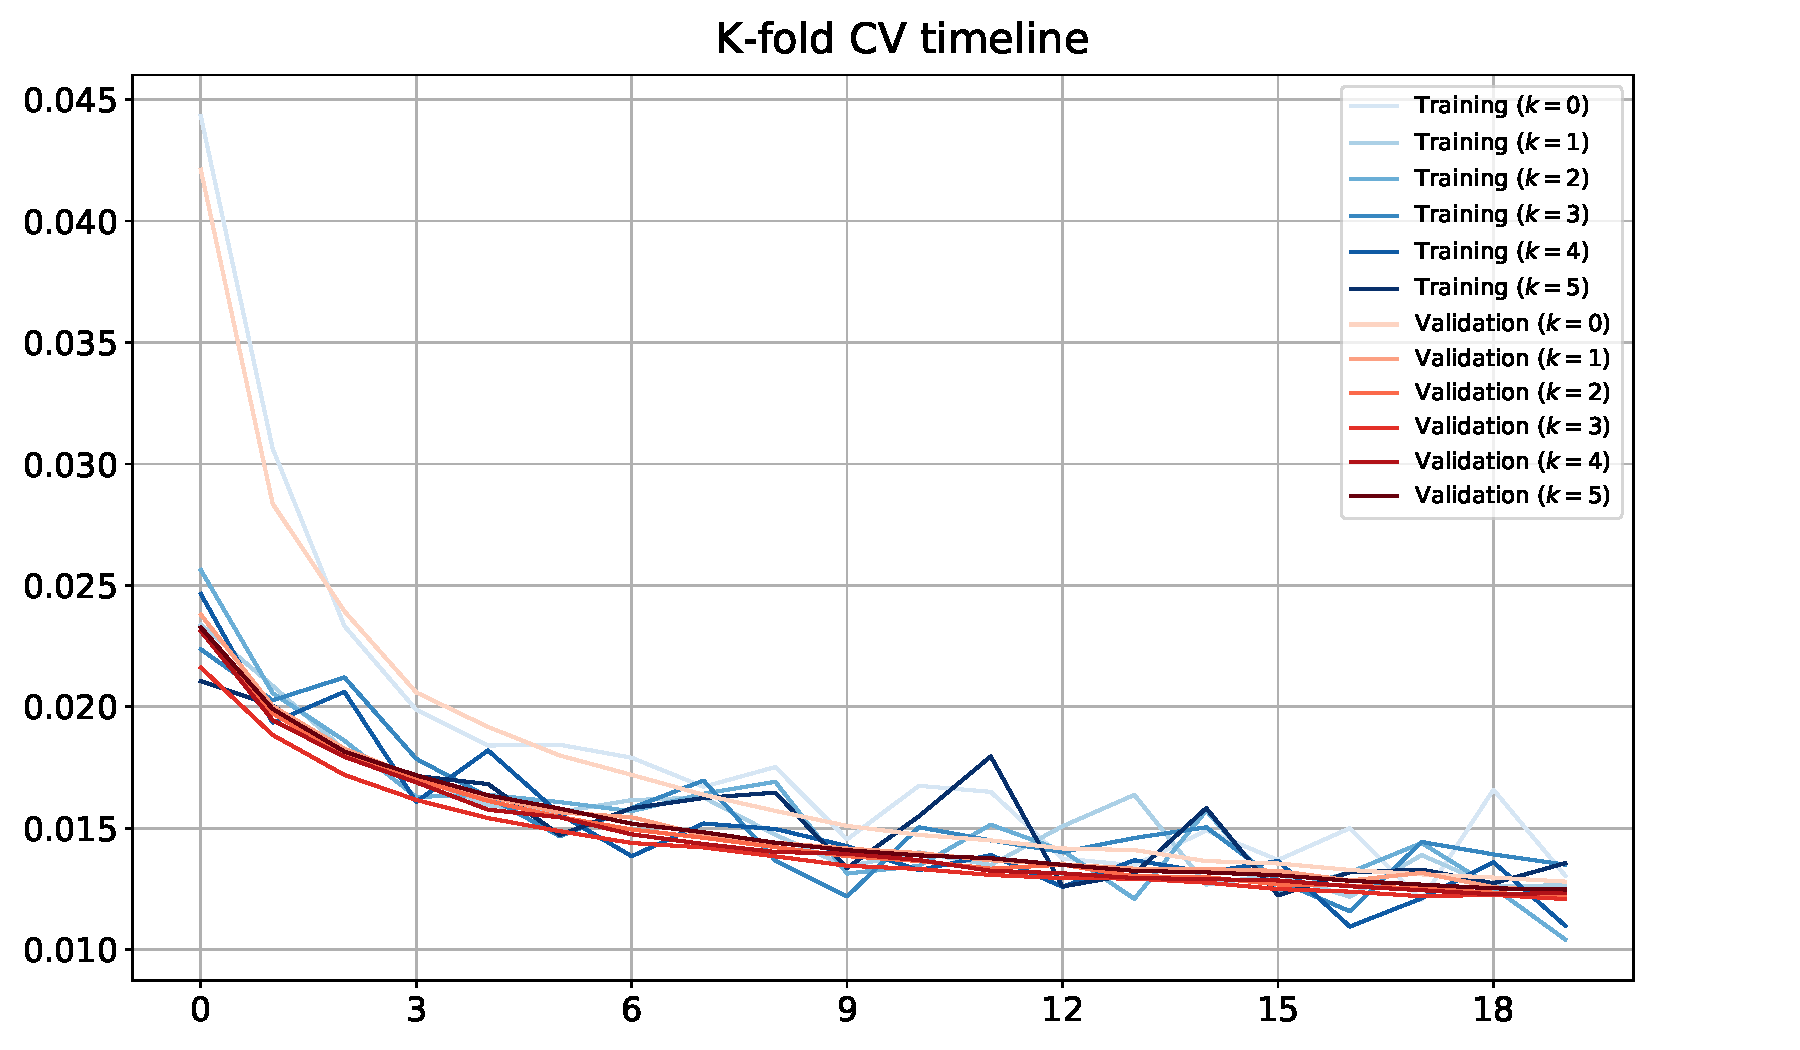
\includegraphics[width=0.7\textwidth]{res/learning_curve_KFCV.pdf}
    \caption{Autoencoder K-fold cross-validation learning curves}
    \label{fig:autoencoder_results}
\end{wrapfigure}

\begin{wraptable}{r}{11cm}
\centering
    \begin{tabular}{ccccccc}
        Layer & \thead{No. channels \\ Neurons} & \thead{(Kernel,\\ Strides,\\ Padding)} & Activation & \thead{Batch \\ Normalization}\\
        \hline
        \textsc{conv1} & 7 & (3, 2, 1) & ReLU & Yes\\
        \textsc{conv2} & 10 & (3, 2, 1) & ReLU & Yes\\
        \textsc{conv3} & 16 & (3, 2, 0) & ReLU & Yes\\
        \textsc{Lin1} & 32 & N/A & ReLU & N/A \\
        \hdashline
        \textsc{Latent} & 3 & N/A & N/A & N/A \\
        \hdashline
        \textsc{Lin1} & 32 & N/A & ReLU & N/A \\
        \textsc{deconv1} & 16 & (3, 2, 0) & ReLU & Yes\\
        \textsc{deconv2} & 10 & (3, 2, 1) & ReLU & Yes\\
        \textsc{deconv3} & 7 & (3, 2, 1) & ReLU & Yes\\
    \end{tabular}
    \caption{Autoencoder architecture. The no. of channels in \textsc{conv[i]} corresponds to output channels, while it corresponds to input channels in \textsc{Deconv[i]}.}
\end{wraptable}
\end{document}